%% Bookheader, Nov 8, 2020; July 18, 2022

\documentclass[11pt]{../Support/ourbook}
%% or for landscape, comment out line above and use this one:
%%\documentclass[landscape,11pt]{ourbook}

%% This will keep space from stretching around display math:

\makeatletter
\renewcommand\normalsize{%
   \@setfontsize\normalsize\@xipt{13.6}%
   \abovedisplayskip 11\p@  \@minus6\p@
   \abovedisplayshortskip \z@ 
   \belowdisplayshortskip 6.5\p@ \@minus3\p@
   \belowdisplayskip \abovedisplayskip
   \let\@listi\@listI}
\makeatother
\normalsize


\begin{document}

\tableofcontents
\graphicspath{{../../Chapters/differentiability/en_US}}
\chapter{Differentiation}

We have done some differentiation, but you haven't been given the real
definition yet, because it is based on limits.

The idea is that we can find the slope between two points on the graph
$a$ and $b$ like this:

$$m = \frac{f(b) - f(a)}{b - a}$$

\begin{figure}[htbp]
    \centering
	\begin{tikzpicture} [scale=2]
	\draw[->,thick,sdkblue] (0,0) -- (4,0) node[right] {$x$};
	\draw[->,thick,sdkblue] (0,0) -- (0, 3.45) node[above] {$y$};
	% curve
	\draw[<->,thick,draw=black, domain=0:3.7,samples=300,variable=\x]  
	plot (\x,{\x * \x * 0.25});
	\draw [sdkblue] (1, 0.25) -- (3, 2.251);
	\draw [dashed] (1,0.25) -- (1, 0) node[below]{$a$};
	\draw [dashed] (3, 2.251) -- (3, 0) node[below]{$b$};
	\draw [dashed] (1,0.25) -- (3, 0.25) node[right] {$f(a)$};
	\draw (3,2.251) node[right] {$f(b)$};
	\draw (1,0.25) circle (0.05);
	\draw (3, 2.251) circle (0.05);
	\draw (2, 0.25) node[above]{$b - a$};
	\draw (3, 1.25) node[right] {$f(b) - f(a)$};
	\end{tikzpicture}
    \caption{The slope of point $a$ using points $a$ and $b$.}
    \label{fig:btoaslope}
\end{figure}

If we want to find the slope at $a$, we take the limit of this as the 
$b$ goes to $a$:

$$f'(a) = \lim_{b \to b}\frac{f(b) - f(a)}{b - a}$$

This idea is usually expressed using $h$ as the difference 
between $b$ and $a$:

\begin{figure}[htbp]
    \centering
	\begin{tikzpicture} [scale=2]
	\draw[->,thick,sdkblue] (0,0) -- (4,0) node[right] {$x$};
	\draw[->,thick,sdkblue] (0,0) -- (0, 3.45) node[above] {$y$};
	% curve
	\draw[<->,thick,draw=black, domain=0:3.7,samples=300,variable=\x]  
	plot (\x,{\x * \x * 0.25});
	\draw [sdkblue] (1, 0.25) -- (3, 2.251);
	\draw [dashed] (1,0.25) -- (1, 0) node[below]{$a$};
	\draw [dashed] (3, 2.251) -- (3, 0) node[below]{$a + h$};
	\draw [dashed] (1,0.25) -- (3, 0.25) node[right] {$f(a)$};
	\draw (3,2.251) node[right] {$f(a + h)$};
	\draw (1,0.25) circle (0.05);
	\draw (3, 2.251) circle (0.05);
	\draw (2, 0.25) node[above]{$h$};
	\draw (3, 1.25) node[right] {$f(a + h) - f(a)$};
	\end{tikzpicture}
    \caption{Limit of a point using $h$ difference.}
    \label{fig:limitSlopeH}
\end{figure}

The formula then becomes:

$$f'(a) = \lim_{h \rightarrow 0}\frac{f(a + h) - f(a)}{h}$$

As $h$ decreases to very close to zero, almost infinitesimal, what we are finding is the sloe of the tangent line to point $a$. 
\begin{figure}[htbp]
    \centering
	\begin{tikzpicture} [scale=2]
	\draw[->,thick,sdkblue] (0,0) -- (4,0) node[right] {$x$};
	\draw[->,thick,sdkblue] (0,0) -- (0, 3.45) node[above] {$y$};
	% curve
	\draw[<->,thick,draw=black, domain=0:3.7,samples=300,variable=\x]  
	plot (\x,{\x * \x * 0.25});
	\draw [sdkblue] (0, -0.25) -- (3, 1.25) node[midway, right]{slope = $f'(a)$};;
	\draw [dashed] (1,0.25) -- (1, 0) node[below]{$a$};
	\draw (1,0.25) circle (0.05);
	\end{tikzpicture}
    \caption{Slope at $a$ as $h$ approaches 0.}
    \label{fig:tangentSlope}
\end{figure}

\section{Differentiability}

Warning: Not every function is differentiable everywhere.  For
example, if $f(x) = |x|$, you get a corner at zero.

\begin{figure}[htbp]
    \centering
	\begin{tikzpicture} [scale=1]
	\draw[->,thick,sdkblue] (-4,0) -- (4,0) node[right] {$x$};
	\draw[->,thick,sdkblue] (0,0) -- (0, 3.45) node[above] {$y$};
	% curve
	\draw[->,thick,draw=black, domain=0:3.7,samples=300,variable=\x]  
	plot (\x,\x);
	\draw[<-,thick,draw=black, domain=-3.7:0,samples=300,variable=\x]  
	plot (\x,{-1 * \x});
	\end{tikzpicture}    
	\caption{Absolute value function.}
    \label{fig:absGraph}
\end{figure}


To the left of zero, the slope is -1. To the right of zero, the slope
is 1.  At zero?  The derivative is not defined because the slopes are two different numbers. 

If a function has a derivative everywhere, it is said to be
\newterm{differentiable}. Generally, you can think of differentiable
functions as smooth --- their graphs have no corners or sharp turns. Another place where a function
is not differentiable is at a vertical tangent, as the slope reaches $\pm \infty$. 

It is important to note: if $f$ is differentiable at $a$, it \emph{must} also be continuous at $a$. 

Likewise, if $f$ is not continuous at $a$ it is not differentiable. An example of this is a jump discontinuity. FIXME diagram here of jump discontinuity. 

\begin{Exercise}[label=diff1]
	[This problem was originally presented as a no-calculator, 
	multiple-choice question on the 2012 AP Calculus BC exam.] Let $f$ 
	be the function defined by $f(x) = \sqrt{|x - 2|}$ for all $x$. 
	Classify each of the following statements as true or false. 
	\begin{enumerate}
		\item $f$ is continuous at $x = 2$. 
		\item $f$ is differentiable at $x = 2$.
		\item $\lim_{x \to 2} f(x) = 0$.
		\item $x = 2$ is a vertical asymptote of the graph of $f(x)$. 
	\end{enumerate}
\end{Exercise}

\begin{Answer}[ref=diff1]
	\begin{enumerate}
		\item True. $f(2)$ exists and $lim_{x \to 2^+}f(x) = 
		\lim_{x \to 2^-}f(x) = f(2) = 0$. 
		\item False. Because of the absolute value, there is a corner in 
		the graph of $f$ at $x=2$. $\lim_{x \to 2^+}f'(x) < 0$ and 
		$\lim_{x \to 2^-}f'(x) < 0$. Therefore there is a discontinuity in 
		$f'(x)$ at $x = 2$ and $f(x)$ is not differentiable at $x = 2$. 
		\item True. $\sqrt{|2-2|} = \sqrt{0} = 0$.
		\item False. $f(2)$ is defined at $x = 2$. 
	\end{enumerate}
\end{Answer}

\section{Using the definition of derivative}

Let's say that you want to know the slope of $f(x) = -3x^2$ at $x = 2$.
Using the definition of the derivative, that would be:

$$f'(2) = \lim_{h \to 0}\frac{f(2 + h) - f(2)}{h} 
= \lim_{h \to 0}\frac{-3(2 + h)^2- \left(-3(2)^2\right)}
{h} $$
$$= \lim_{h \to 0}\frac{-12 - 12h + 
-3(h)^2 + 12}{h} = -12$$ 



\graphicspath{{../../Chapters/derivative_definition/en_US}}
\chapter{Derivatives}

In calculus, the derivative of a function represents the rate at which
the function is changing at a particular point. It is a fundamental
concept that has vast applications in various fields, including
physics.\index{derivative}

\section{Definition}

The derivative of a function $f(x)$ at a point $x$ is defined as the limit:

\begin{equation}
f'(x) = \lim_{{h \to 0}} \frac{f(x+h) - f(x)}{h}
\end{equation}

provided this limit exists. In words, the derivative of $f$ at $x$ is
the limit of the rate of change of $f$ at $x$ as the change in $x$
approaches zero.

\section{Applications in Mathematics}
\subsection{l'Hospital's Rule}
Consider the function $h(x) = \frac{\ln{x}}{x-1}$ and suppose we are interested in the behavior of $h(x)$ around $x=1$. If we apply the Quotient Rule, we get an indeterminate result: $$\lim_{x \to 1}\frac{\ln{x}}{x-1} = \frac{0}{0}$$ Looking at the graph of $h(x)$, we can guess that $\lim_{x \to 1}\frac{\ln{x}}{x-1} = 1$. 

\begin{tikzpicture}
\begin{axis}
    [clip=true,
    xmin=0, xmax=4,
    ymin=0, ymax=4,
    axis lines=left
    ]
    \addplot[blue, domain=0.01:4, samples=100]{ln(x)/(x-1)};
    \addplot[samples=50, black, dashed] coordinates{(1, 0)(1,1)};
    \addplot[samples=50, black, dashed] coordinates{(0, 1)(1,1)};
    \addplot[mark=*, fill=white, draw=blue] coordinates{(1, 1)};
\end{axis}
\end{tikzpicture}

Let's examine the numerator and denominator separately: we'll define $f(x)=\ln{x}$ and $g(x) = x-1$. 

\begin{tikzpicture}
    \begin{axis}
    [clip=false,
    xmin=0, xmax=3,
    ymin=-1, ymax=2,
    axis lines = center]
    \addplot[blue, samples=100, domain=1/e:3]{ln(x)}
    node[right, pos=1]{$f(x)$};
    \addplot[red, samples=100, domain=0:3]{x-1}
    node[right, pos=1]{$g(x)$};
    \end{axis}
\end{tikzpicture}

If we zoom in very far around $x=1$, the graphs begin to look linear:

\begin{tikzpicture}
    \begin{axis}
    [clip=false,
    xmin=0.9, xmax=1.1,
    ymin=-0.1, ymax=0.1,
    axis lines = center]
    \addplot[blue, samples=100, domain=0.9:1.1]{ln(x)}
    node[right, pos=0.9]{$f(x)$};
    \addplot[red, samples=100, domain=0.9:1.1]{x-1}
    node[right, pos=1]{$g(x)$};
    \end{axis}
\end{tikzpicture}

We can approximate these graphs as linear functions with slopes $m_1$ and $m_2$, so that the blue curve is approximated as $y=m_1(x-1)$ and the red curve is approximated as $y=m_2(x-1)$. The ratio of the functions would then be $$\frac{m_1(x-1)}{m_2(x-1)}=\frac{m_1}{m_2}$$ which is the same as the ratio of the derivatives of our linear approximations. This suggests l'Hospital's rule, that the limit of a ratio is the same as the limit of the ratio of the derivatives for certain indeterminate forms: $$\lim_{x\to a}\frac{f(x)}{g(x}=\lim_{x\to a}\frac{f'(x)}{g'(x)}$$.

Let's apply l'Hospital's rule to our limit of $h(x)$:
$$\lim_{x\to 1}\frac{\ln{x}}{x-1}=\lim_{x \to 1}\frac{\frac{d}{dx}\ln{x}}{\frac{d}{dx}(x-1)}=\lim_{x \to 1}\frac{\frac{1}{x}}{1}=1$$

Notice our result with l'Hospital's rule matches our guess based on the graph of $h(x) = \frac{\ln{x}}{x-1}$. 

L'Hospital's rule also applies to the indeterminate result $\frac{\pm \infty}{\pm \infty}$. For a limit of the form $\lim_{x\to a}\frac{f(x)}{g(x)}$, l'Hospital's rule applies if:
\begin{enumerate}
    \item the original limit is of the indeterminate form $\frac{0}{0}$ or $\frac{\pm \infty}{\pm \infty}$
    \item $f$ and $g$ are differentiable on an interval containing $a$ (but possibly not differentiable at $a$)
    \item $g'(x) \neq 0$ on said interval
\end{enumerate}

\subsection{Intervals of Increasing and Decreasing Value}
\subsubsection{Practice}
\begin{Exercise}
    [label=incdec1]
    Let $f$ be the function given by $f(x) = 300x-x^3$. On which of the following intervals is $f$ increasing?
\end{Exercise}
\begin{Answer}
    [ref=incdec1]
    First, we will find $f'$ and set it equal to zero: $$f'(x)=300-3x^2=0$$ $$300=3x^2 \rightarrow x=\pm \sqrt{100} = \pm10$$ Now we will evaluate the value of $f'(x)$ for $x<-10$, $-10<x<10$, and $x>10$. 
    \begin{center}
        \begin{tabular}{c|c|c}
        Value of $x$ & Computation & $f(x)$ increasing or decreasing?\\
         $x<-10$    &  $300-3(-11)^2<0$ & decreasing\\
         $-10<x<10$    & $300-3(0)^2>0 $ & increasing\\
         $x>10$&$300-3(11)^2<0$& decreasing
        \end{tabular}
    \end{center}
    Therefore, the fucntion is increasing on the interval $x \in [-10, 10]$ because $f'(x) >0$ for $x \in [-10, 10]$.
\end{Answer}

\subsection{Mean Value Theorem}

The Mean Value Theorem (MVT) states that on an interval $[a, b]$ where a continuous function $f$ is differentiable on an open interval $(a, b)$, there is at least one point where the tangent line to $f$ has the same slope as a line connecting the points $(a, f(a))$ and $(b, f(b))$. Consider the graph of $f(x) = x^2$ below. The line connecting the points $(-1, 1)$ and $(2, 4)$ has a slope of $\frac{1}{2}$. MVT tells us there must be \textit{at least one} point, $c$, on the interval $x \in (-1, 2)$ where $f'(c) = \frac{1}{2}$. We can find this point by setting $f'(x)$ equal to $\frac{1}{2}$: $$2x=\frac{1}{2} \rightarrow x=\frac{1}{4}$$

Examining the graph, you can see that the tangent at $f(\frac{1}{4})$ (the black line) is parallel to the line connecting $(-1, f(-1))$ and $(2, f(2))$. 

\begin{tikzpicture}
    \begin{axis}
        [ymin=-2, xmin=-2, xmax=2, axis lines = left]
        \addplot[blue, samples=50]{x^2};
        \addplot[red, mark=*]coordinates {(-1, 1)};
        \addplot[red, mark=*] coordinates {(2, 4)};
        \addplot[domain=-2:2, red] coordinates{(-1, 1)(2, 4)};
        \addplot[black, mark=*] coordinates{(0.5, 0.25)};
        \addplot[black, domain=-2:2, samples=50
        ]{x-0.25};
    \end{axis}
\end{tikzpicture}

Note that MVT doesn't tell us \textit{where} $f'(x)$ is parallel to the line connecting $(a, f(a))$ and $(b, f(b))$, just that some value $c$ exists that satisfies the condition. 

Consider a hammer thrown upwards at 5 $\frac{m}{s^2}$ on Earth (where the acceleration due to gravity is approximately $-9.8 \frac{m}{s^2}$). We can use MVT to show that there must be some point in the hammer's path upwards where the velocity of the hammer is exactly equal to its average velocity as it flies through the air. 
The hammer's rise can be described with the function $y(t) = 5t-4.9t^2$. The hammer reaches its peak at approximately $t=0.51$. So, we are looking for some value, $c$, such that $$y'(c) = \frac{y(0.51)-y(0)}{0.51-0}=\frac{5(0.51)-4.9(0.51^2)}{0.51}=\frac{1.2755}{0.51}=2.5$$

Solving $y'(t) = 5-9.8t = 2.5$, we find that the $c$ that satisfies MVT is approximately $0.255$. This result is illustrated on the graph below:

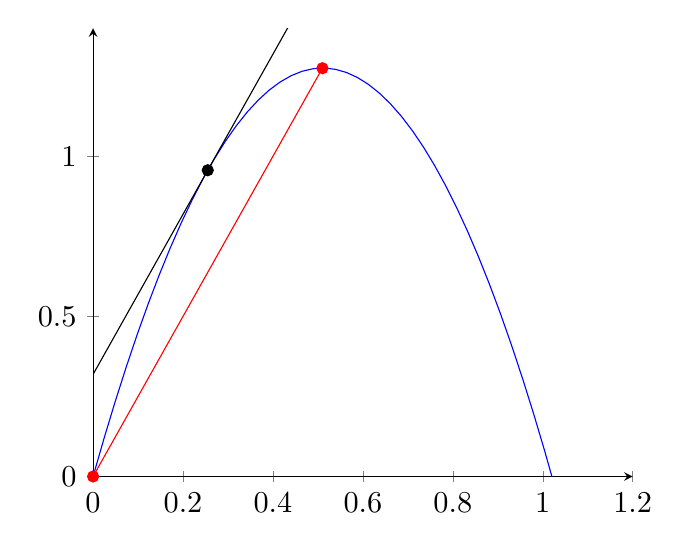
\begin{tikzpicture}
    \begin{axis}[ymin=0,ymax=1.4, xmin=0, xmax=1.2, axis lines=left]
    \addplot[blue, samples=50, domain=0:1.2]{5*x-4.9*x^2};
    \addplot[mark=*, red] coordinates{(0,0)};
    \addplot[mark=*, red] coordinates{(0.51, 1.275)};
    \addplot[red, samples=50]coordinates{(0,0) (0.51, 1.275)};
    \addplot[black, samples=50]{2.5*(x-0.255)+0.9564};
    \addplot[mark=*, black]coordinates{(0.255, 0.9564)};
    \end{axis}
\end{tikzpicture}

\subsubsection{MVT Practice}
\begin{Exercise}
[label=MVT1]
AT 3:30 PM, a car's speedometer reads $30 \frac{mi}{hr}$. At 3:40 PM, it reads $50\frac{mi}{hr}$. Show that at some time between 3:30 and 3:340 PM, the car's acceleration is exactly $120 \frac{mi}{hr^2}$. 
\end{Exercise}
\begin{Answer}
[ref=MVT1]
The speed of a car must a continuous, differentiable function, since your car can't "jump" from one speed to another: it must smoothly accelerate from one speed to another. Therefore, the Mean Value Theorem applies. The average acceleration from 3:30 PM to 3:40 PM is given by:
$$\frac{\text{change in speed}}{\text{change in time}} = \frac{50 \frac{mi}{hr}-30\frac{mi}{hr}}{3:40PM-3:30PM}$$ 
Simplifying and converting minutes to hours, we see the average acceleration is:
$$\frac{20\frac{mi}{hr}}{\frac{1}{6}hr} = 120\frac{mi}{hr^2}$$

Therefore, by MVT, there must be some time between 3:30 and 3:40 PM where the car's acceleration is exactly $120 \frac{mi}{hr^2}$. 
\end{Answer}

\begin{Exercise}
[label=MVT2]
Find the number $c$ that satisfies the MVT on the given interval. 

(a) $f(x) = \sqrt{x}$, $[0, 4]$

(b)$f(x) = e^{-x}$, $[0,2]$

(c)$f(x) = \ln{x}$, $[1,4]$	
\end{Exercise}

\begin{Answer}
[ref=MVT2]
(a) For the domain given, $f(x)$ is defined and differentiable. Finding the slope of the secant line connecting the endpoints:
$$\frac{f(b)-f(a)}{b-a}=\frac{\sqrt{4}-\sqrt{0}}{4-0}=\frac{2}{4}=\frac{1}{2}$$
So we are looking for some number $c$ such that $f'(c) = \frac{1}{2}$. Let's find $f'(x)$:
$$f'(x) = \frac{d}{dx}\sqrt{x}=\frac{1}{2\sqrt{x}}$$
Setting this equal to $\frac{1}{2}$ to find $c$:
$$f'(c) = \frac{1}{2\sqrt{c}}=\frac{1}{2}$$
$$\sqrt{c}=1$$
$$c=1$$

(b)For the domain given, $f(x)$ is defined and differentiable. Finding the slope of the secant line connecting the endpoints:
$$\frac{f(2)-f(0)}{2-0}=\frac{e^{-2}-e^{0}}{2}=\frac{1-e^{2}}{2e^{2}}\approx -0.432$$
And find $f'(x)$:
$$f'(x) = -e^{-x}$$
According to MVT, there must be some $c$ such that $f'(c) \approx-0.432$:
$$-e^{-c} \approx -0.432$$
$$e^{-c}\approx 0.432$$
$$-c \approx \ln{0.432}$$
$$c \approx -\ln{0.432} \approx 0.839$$

(c) For the domain given, $f(x)$ is defined and differentiable. Finding the secant line connecting the endpoints:
$$\frac{f(b)-f(a)}{b-a}=\frac{\ln{4}-\ln{1}}{4-1}=\frac{\ln{4}}{3}\approx 0.462$$
And find $f'(x)$:
$$f'(x) = \frac{1}{x}$$
According to MVT, there must be some $c$ such that $f'(c) \approx 0.462$
$$f'(c) = \frac{1}{c} \approx 0.462$$
$$c \approx \frac{1}{0.462} = 2.164$$
\end{Answer}

\section{Applications in Physics}

In physics, derivatives play a vital role in describing how quantities
change with respect to one another.

\subsection{Velocity and Acceleration}

In kinematics, the derivative of the position function with respect to
time gives the velocity function, and further taking the derivative of
the velocity function gives the acceleration function. For example, if
$s(t)$ represents the position of an object at time $t$, then the
velocity $v(t)$ and acceleration $a(t)$ are given by:

\begin{equation}
v(t) = \frac{ds}{dt} \quad \text{and} \quad a(t) = \frac{dv}{dt} = \frac{d^2s}{dt^2}
\end{equation}

\subsection{Force and Momentum}

In mechanics, the derivative of the momentum of an object with respect
to time gives the net force acting on the object, as stated by
Newton's second law of motion:

\begin{equation}
F = \frac{dp}{dt}
\end{equation}

where $F$ is the force, $p$ is the momentum, and $t$ is the time.


\graphicspath{{../../Chapters/derivative_rules/en_US}}
\chapter{Rules for Finding Derivatives}

\graphicspath{{../../Chapters/optimization/en_US}}
\chapter{Optimization}

Optimization is a branch of mathematics that involves finding the best solution from all feasible solutions. In the field of operations research, optimization plays a crucial role. Whether it is minimizing costs, maximizing profits, or reducing the time taken to perform a task, optimization techniques are employed to make decisions effectively and efficiently.

\section{Optimization Problems}
An optimization problem consists of maximizing or minimizing a real function by systematically choosing the values of real or integer variables from within an allowed set. This function is known as the objective function.

A standard form of an optimization problem is:

\begin{equation*}
\begin{aligned}
& \underset{x}{\text{minimize}}
& & f(x) \
& \text{subject to}
& & g_i(x) \leq 0, ; i = 1, \ldots, m \
&
& & h_j(x) = 0, ; j = 1, \ldots, p
\end{aligned}
\end{equation*}

where
\begin{itemize}
\item $f(x)$ is the objective function,
\item $g_i(x) \leq 0$ are the inequality constraints,
\item $h_j(x) = 0$ are the equality constraints.
\end{itemize}

\section{Types of Optimization Problems}
There are different types of optimization problems, including but not limited to:

\begin{itemize}
\item \textbf{Linear Programming:} The objective function and the constraints are all linear.
\item \textbf{Integer Programming:} The solution space is restricted to integer values.
\item \textbf{Nonlinear Programming:} The objective function and/or the constraints are nonlinear.
\item \textbf{Stochastic Programming:} The objective function and/or constraints involve random variables.
\end{itemize}

These problems are solved using different techniques and algorithms, many of which are a subject of active research.

\section{Applications}
Optimization techniques have a wide variety of applications in many fields such as economics, engineering, transportation, and scheduling problems.


%%%%%%%%%%%%%%%%%%%%%%%%%%%%%%%%%
%% Bookfooter.tex by Aaron Hillegass
%% Nov 8, 2020

\appendix

\chapter{Answers to Exercises}
\shipoutAnswer

\bibliography{references}

\printindex

\end{document}